\subsection{Simulación con LTSpice}

La simulación de LTSpice de la fig. \ref{fig:2:ltspice} del amplificador no
inversor de la fig. \ref{fig:2:esquema} arrojó una ganancia $A = 2.304$ en
todos los casos, que concuerda con el análisis teórico. El único factor que
varió fue la corriente $I_{R_L}$, de $0.4413$, $2.074$ y
$\SI{20.74}{\milli\ampere}$ para las resistencias de $47$, $10$ y 
$\SI{1}{\kilo\ohm}$.

Para el amplificador seguidor de tensión se simuló el circuito de la fig.
\ref{fig:2:esquema-seguidor} con LTSpice, según lo indicado en la fig.
\ref{fig:2:ltspice-seguidor}. En todos los casos se obtuvo una ganancia $A=0.998$, que
concuerda con lo visto en la sección anterior. La única variable que presentó
diferencias según el valor de $R_L$ que se utilizara fue, por supuesto, la 
corriente por dicho resistor, de $0.1911$, $0.8984$ y
$\SI{8.984}{\milli\ampere}$ para resistencias de $47$, $10$ y
$\SI{1}{\kilo\ohm}$, respectivamente.

\begin{figure}[H]
    \centering
    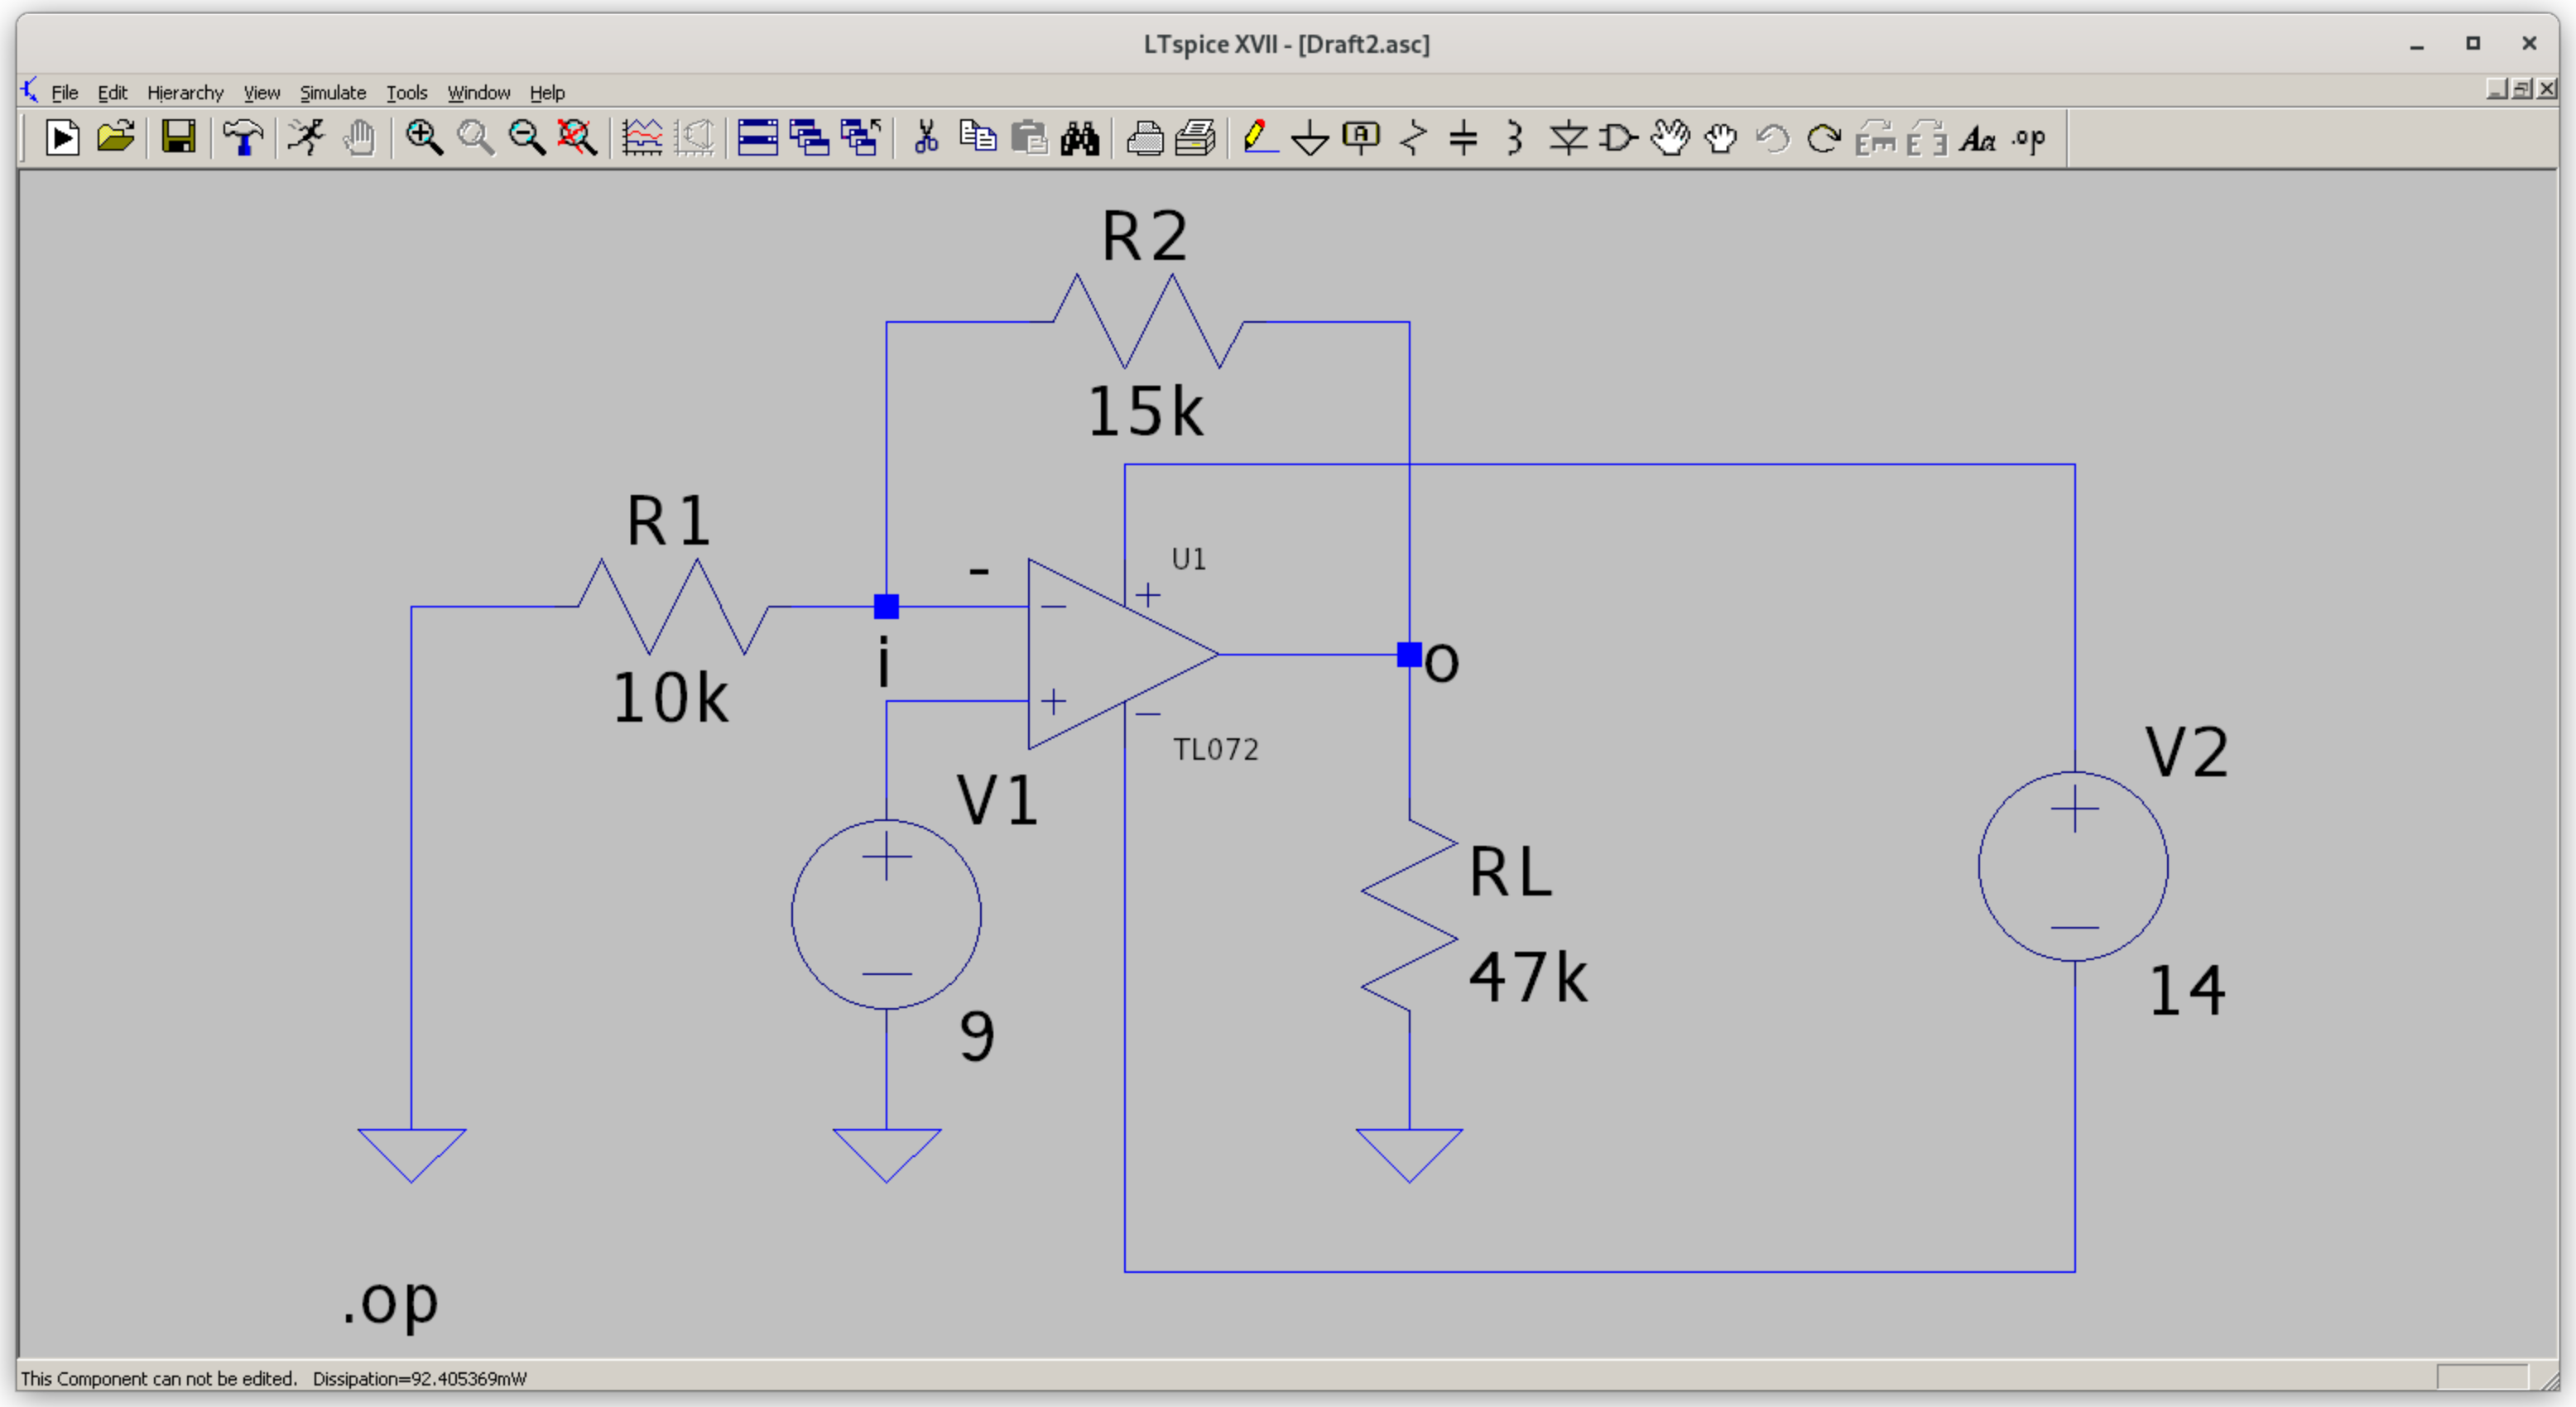
\includegraphics[width=0.8\textwidth]{img/2/ltspice.png}
    \caption{Simulación en LTSpice del circuito de la fig. \ref{fig:2:esquema}}
    \label{fig:2:ltspice}
\end{figure}

\begin{figure}[H]
    \centering
    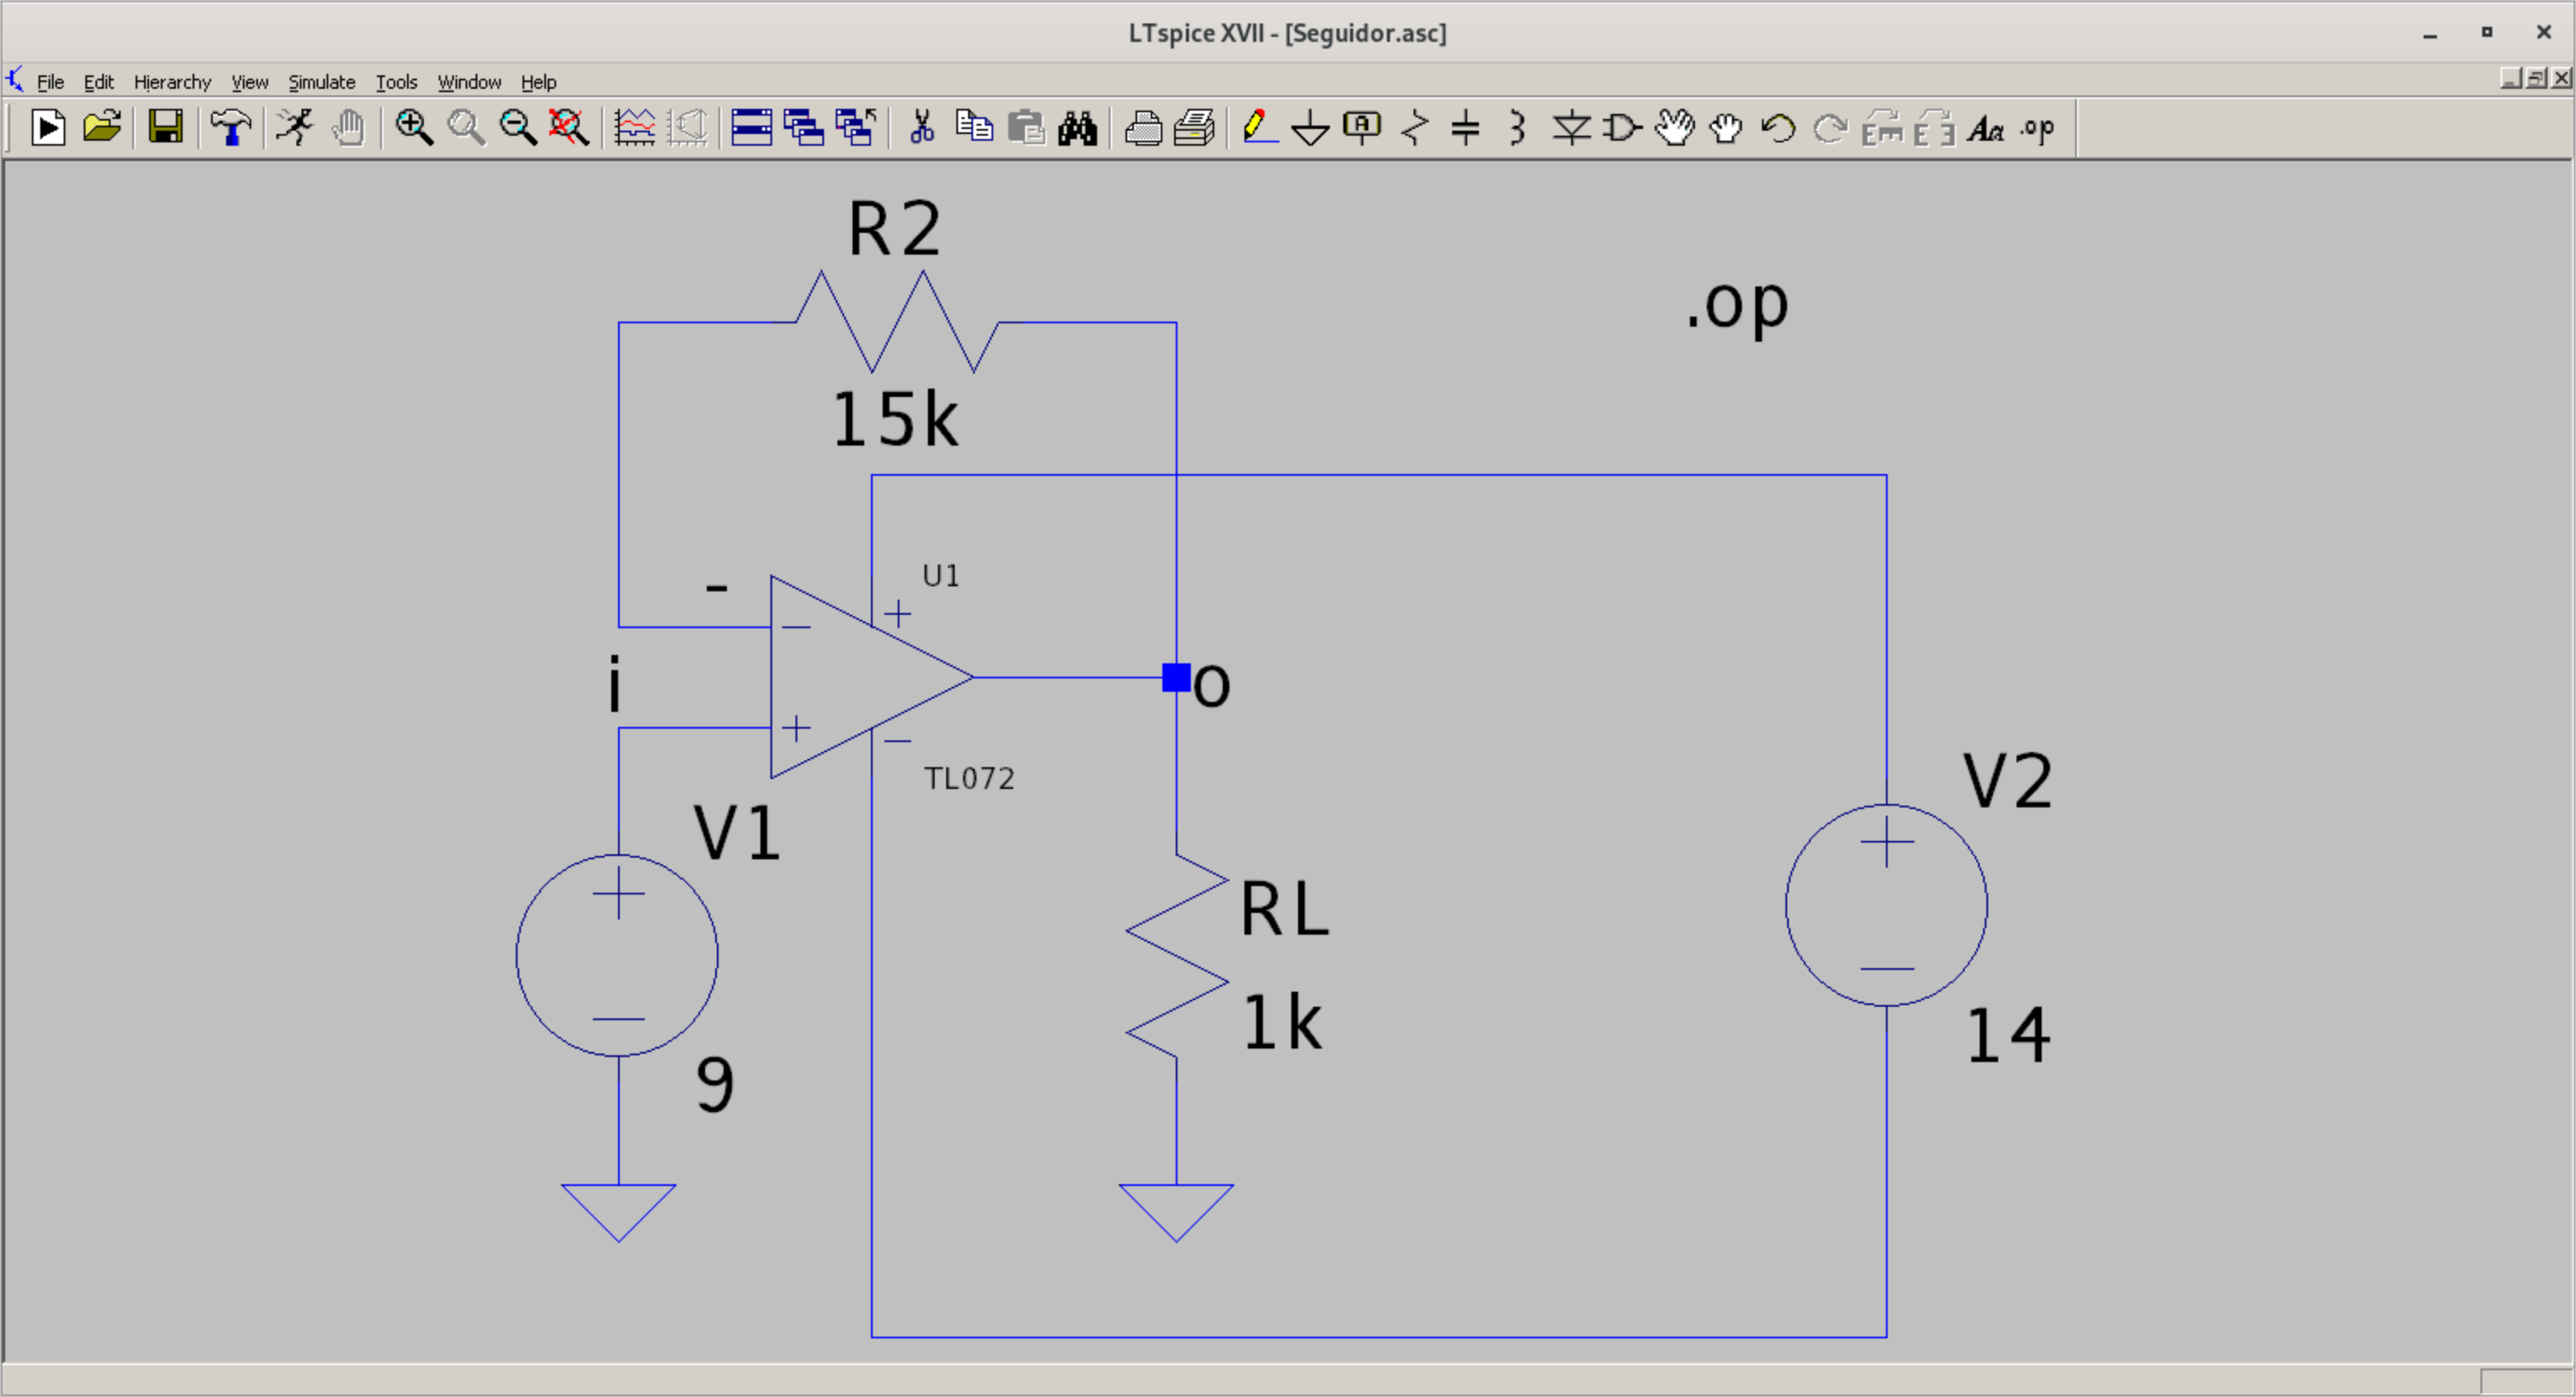
\includegraphics[width=0.8\textwidth]{img/2/ltspice-seguidor.png}
    \caption{Simulación en LTSpice del circuito de la fig.
        \ref{fig:2:esquema-seguidor}}
    \label{fig:2:ltspice-seguidor}
\end{figure}
